\mainchapter{Background Theory}{0.6}{Research is to see what everybody else has seen, and think what nobody else has thought.}{Arthur Schopenhauer} \label{chap:theory}

%----------------------------------------%
% Background Theory
%----------------------------------------%

This chapter introduces the key concepts and theories required to better appreciate the work and the results presented in this thesis. We start with an introduction to fluid mechanics, essential to the description of stellar interiors and supernova explosions (\Cref{sec:fluid_mech}). We then broadly discuss the theory describing the formation of stars and their subsequent evolution onto the main sequence (\Cref{sec:stellar_evo}) before moving on to a more central part of this thesis, namely supernovae (\Cref{sec:sne}). We then discuss the field of numerical simulations applied to core-collapse supernovae (\Cref{sec:sims}), and present the concept of neutrino-driven winds (\Cref{sec:ndw}).

\section{Fluid mechanics} \label{sec:fluid_mech}

The vast majority of the atoms and molecules, composing the baryonic matter in the universe, are not held tightly together as they would be in a solid, but are rather in the form of freely floating particles, interacting between one another through collisions, electromagnetic forces and other such processes. We aim to construct a model that allows us to describe the motion of such fluids of microscopic particles, so as to predict its macroscopic evolution, and do so in a way that can be solved numerically.

Ideally, we would want to resolve the complete quantum mechanical state of each particle in the system and their interactions, but this would clearly be too complicated to express mathematically, and prohibitively expensive to solve from a numerical point of view. For example, in a star, where as many as \(10^{20}\ \mathrm{particles/cm^{3}}\) can be found just on its surface, we cannot reasonably consider evaluating the microscopic properties and behaviour of each individual particle. However, we can realise that a single particle will have an almost negligible impact on the evolution of the entire system, which is rather dictated by the collective behaviour of all the particles together. Considering the system as a whole, we can derive relevant macroscopic quantities such as density, pressure and temperature, as statistical averages of the properties of the particles in the system. Manifestly, averaging over an entire star would not be very helpful, and would reduce the problem to that of a uniform, spherical cow. But we can average over locally equilibrated regions of the fluid and, under reasonable assumptions, consider these regions to be infinitesimally small so as to treat our system as a continuum.

This idea is the foundation of fluid mechanics, and is an essential theory for the description of the dynamics of matter in the Universe. We note however that, in contrast with standard terrestrial fluid mechanics, the treatment of fluids in an astrophysical context harbours some key differences. This mainly stems from the fact that fluids in the Universe are rarely in a liquid state, either due to very low density environments, or extremely high temperatures. We are therefore more interested in the gaseous and plasma phases of the fluid. The consequence is that we cannot assume the fluid to be incompressible, as we would do with e.g. liquid water on Earth, and we must consider flows that can be accelerated to supersonic velocities as well.

In the following sections, we further describe the key principles and assumptions of fluid mechanics in an astrophysical context, and derive the hydrodynamic equations. %that we extend for the treatment of plasmas, giving the magnetohydrodynamic equations.
The derivations presented here are based on \cite{Clarke2007}. 

\subsection{Fluid element} \label{sec:fluid_elem}

We build our fluid by considering a continuum of infinitesimally small, locally equilibrated portions of it, that we now refer to as \emph{fluid elements}. This concept allows us to define local macroscopic quantities, that corresponds to statistical averages of the properties of the particles contained in a fluid element, the main of which are described below.

\begin{description}
    \item[Density] We simply consider the number of particles contained in a fluid element. Divided by the volume, it gives the average number of particles that we expect to find in a unit of volume, or number density, usually termed \(n\). Multiplying by the average mass of a particle in the fluid yields the mass density, noted \(\rho\).

    \item[Velocity] The particles in the fluid each have a velocity. Averaging these velocities gives the flow velocity \(\fvec{u}\), which simply describes how the fluid moves as a whole.

    \item[Temperature] The deviation of each particle's velocity from the flow velocity gives a chaotic motion component that we can assume to be drawn from a statistical distribution (typically Maxwell-Boltzmann distribution for an ideal gas). Because it is a random distribution, the velocities would average to zero, and so we rather average their magnitudes to reflect the temperature \(T\) of the fluid, or how much chaotic motion there is in the fluid.

    \item[Internal energy] How much energy is contained in the fluid is quantified by the internal energy \(\mathcal{E}\). This energy can be in the form of translational kinetic energy of particles, as quantified by the temperature, but encompasses many other forms as well: vibrational and rotational kinetic energy, in the case of certain molecules; energy from nuclear processes such as fusion or fission; energy from excited or ionised electrons; and energy from electromagnetic interactions between particles. From a hydrodynamic perspective, energy is a conserved quantity, and is therefore more important than temperature, as will be shown later in this section.

    \item[Pressure] Lastly, we consider the interaction between particles through collisions. Each particle may collide with another, reflecting their momentum in the other direction, as if bouncing off a solid surface. This can be approximated by a force applied by the surface to the particle to send it in the other direction. Averaging this force over many collisions gives the pressure \(P\), and quantifies how strongly the particles interact.
\end{description}

In order to define these quantities, we must put some constraints on the actual size of a fluid element. If we symbolise the size of the fluid element by \(s\), we must have that

\begin{enumerate}
    \item the fluid element is much smaller than the scale length for change of any relevant quantity \(Q\),
    \begin{equation}
        s \ll \frac{Q}{|\nablavec Q|} \punct{.}
    \end{equation}

    \item the fluid element is large enough to contain a statistically relevant number of particle. So that if we write \(n\) the number density of particles, we have
    \begin{equation}
        n s^3 \gg 1 \punct{.}
    \end{equation}

    \item the fluid element is much larger than the mean free path \(\lambda\) of a particle,
    \begin{equation}
        s \gg \lambda \punct{.}
    \end{equation}
\end{enumerate}

The first of these constraints guarantees the continuity of the macroscopic quantities describing the fluid. The second, that these quantities accurately describe the macroscopic behaviour of the fluid, away from any fluctuations, or noise, caused by the finite number of particles. The third and final condition ensures that the interactions between particles occur often enough that the element is in \emph{Local Thermodynamic Equilibrium} (LTE), meaning that it has a well-defined distribution of particle velocities. Clearly, this last criterion can only apply to collisional systems, and will allow us to derive an equation of state. But although collisionless fluids do exist, they are not relevant for this work and we therefore disregard them.

\subsection{Eulerian \& Lagrangian formalism} \label{sec:fluid_form}

The concept of a fluid element gives us a framework from which we can derive equations expressing the evolution of the system over time. But which system are we describing; a single fluid element or the fluid as a whole? In reality, these two possible approaches describe two competing formalisms, known as the Eulerian and the Lagrangian formalism.

\begin{description}
    \item[Eulerian description] We formulate the equations considering the fluid as a whole, in which each fluid element is fixed in space and the fluid flows through them. A quantity, for example the density, would be expressed as both a function of position \(\fvec{r}\) and time \(t\), \(\rho = \rho(\fvec{r}, t)\), and we express its time derivative using the symbol \(\partial_t\), thus evaluated at a fixed position \(\fvec{r}\).
    
    \item[Lagrangian description] We instead formulate the equations in the frame of reference of a single fluid element, that moves with the flow, and look at the changes of the variables within that element, as it is advected by the fluid. A coordinate system such as in the Eulerian description becomes irrelevant, and we rather express quantities as a function of time \(t\) and a label \(l\), referring to a certain fluid element, \(\rho = \rho(l, t)\). Using this formulation, we instead express the time derivative using the symbol \(D_t\), and is evaluated within a fluid element, in a coordinate system comoving with the fluid.
\end{description}

Clearly, the two formulations only differ by their relation with the flow velocity. Thus, we should be able to jump from Eulerian to Lagrangian description by accounting for the spatial gradient of any considered quantity \(Q\) in the direction of the flow, reflecting the change of the variable as the fluid element moves to a new location. Here we give the relationship connecting Eulerian and Lagrangian formulations, and refer the reader to \cite{Clarke2007} for a more descriptive derivation.
\begin{equation}
    D_t Q = \partial_t Q + \fvec{u} \cdot \nablavec Q \punct{.} \label{eq:eul_to_lag}
\end{equation}

\subsection{Hydrodynamic equations} \label{sec:fluid_eqs}

We have demonstrated that we can represent our fluid of microscopic particles as continuous fields of macroscopic, thermodynamic quantities. From the property of continuity, and as is customary in classical mechanics, we can derive equations known as conservation laws to formulate the evolution of these fields. These laws simply express that the rate of change of any given quantity within a fluid element must be balanced by the net flow through this element, sources and sinks, and interactions from outside. We use this concept to express the conservation of mass, momentum and energy.

\subsubsection{Conservation of mass} \label{sec:fluid_eq_mass}

Starting with the conservation of mass, it is natural to expect that, in the absence of any source or sink, the rate of change of mass within a volume element must be balanced by the amount of mass entering or leaving this volume.

It is perhaps simpler to derive mass conservation from a Eulerian perspective, at a fixed location in the fluid. Thus, we consider a fixed volume \(V\), of volume element \(\upd[V]\), whose surface \(S\) has surface element \(\updvec{S} = \fvec{n}\,\upd[S]\), where \(\fvec{n}\) is a vector of unit length, normal to the surface and pointing outward from the enclosed volume.

Then, the total mass must be the density integrated over the volume, and taking the time derivative of this quantity gives the rate of change of mass
\begin{equation}
    \partial_t \int_V \rho\,\upd[V] \punct{.} \label{eq:mass_change}
\end{equation}

The net flow of mass through the volume can be expressed as the flux of mass passing through the surface, giving
\begin{equation}
    - \int_S \rho \fvec{u} \cdot \updvec{S} = - \int_V \nablavec \cdot (\rho \fvec{u}) \upd[V] \punct{,} \label{eq:mass_flux}
\end{equation}

where we used the divergence theorem to write a volume integral and, because \(\updvec{S}\) points outwards, we added a minus sign in order to get the mass inflow. Then, equating \ref{eq:mass_change} with \ref{eq:mass_flux} gives
\begin{equation}
    \partial_t \int_V \rho\,\upd[V] = - \int_V \nablavec \cdot (\rho \fvec{u}) \upd[V] \punct{.}
\end{equation}

Because this relation is true for all the volumes, we can simply write
\begin{boxedeq}
    \begin{equation}
        \textit{Conservation of mass (Eulerian)} \qquad \partial_t \rho + \nablavec \cdot (\rho \fvec{u}) = 0 \punct{,} \label{eq:mass_eul}
    \end{equation}
\end{boxedeq}

which is the Eulerian form for mass conservation. It can be rewritten in Lagrangian form using \Cref{eq:eul_to_lag},
\begin{boxedeq}
    \begin{equation}
        \textit{Conservation of mass (Lagrangian)} \qquad D_t \rho + \rho \nablavec \cdot \fvec{u} = 0 \punct{.} \label{eq:mass_lag}
    \end{equation}
\end{boxedeq}

\subsubsection{Conservation of momentum} \label{sec:fluid_eq_mom}

Next, conservation of momentum, is in fact Newton's second law of motion,
\begin{equation}
    \fvec{F} = D_t \fvec{p} = D_t \left( \int_V \rho \fvec{u} \,\upd[V] \right) \punct{.} \label{eq:newton2}
\end{equation}

Here, we consider the external forces acting on a single fluid element, of volume \(V\), with momentum \(\fvec{p} = \int_V \rho \fvec{u} \,\upd[V]\). For one part, it is common to generalise the total force acting on the system as a sum of body forces, acting on the entire volume, and surface forces, only interacting through the surface of the volume. The rate of change of momentum then becomes
\begin{equation}
    D_t \left( \int_V \rho \fvec{u} \,\upd[V] \right) = \int_S \fvec{\sigma} \cdot \updvec{S} + \int_V \rho \fvec{f} \,\upd[V] \punct{.}
\end{equation}

In this expression, \(\fvec{f}\) represents the body forces, and is an acceleration field representing forces arising from, for example, gravity. Therefore, we may write
\begin{equation}
    \fvec{f} = \fvec{g} = - \nablavec \phi \punct{,}
\end{equation}

where \(\fvec{g}\) is the gravitational acceleration, and \(\phi\) the gravitational potential.

Next, \(\fvec{\sigma}\) is defined as the stress tensor. In simple terms, the components \(\sigma_{ij}\) of the stress tensor gives the force in the direction \(i\) acting on a surface whose normal is in the direction \(j\). It encompasses forces acting on the surface of the volume considered, such as thermal pressure, viscous stresses and magnetic pressure. We only consider the thermal pressure for the following derivation, excluding magnetic forces and viscosity.

The pressure \(P\) acting on a surface element \(\updvec{S}\) is \(-P\updvec{S}\), where again we must add a minus sign as the surface element \(\updvec{S}\) is directed outward, but the pressure force must be acting inwards. If we only consider the component of the force in the direction of an arbitrary unit vector \(\unitvec{n}\), we can again make use of the divergence theorem to write
\begin{align}
    F & = - \int_S P \unitvec{n} \cdot \updvec{S} \nonumber \\
      & = - \int_V \nablavec \cdot (P\unitvec{n}) \upd[V] \punct{.}
\end{align}

Newton's equation of motion in the direction of \(\unitvec{n}\) can then be written as
\begin{equation}
    D_t \left( \int_V \rho \fvec{u} \,\upd[V] \right) \cdot \unitvec{n} = - \int_V \nablavec \cdot \left( P\unitvec{n} \right) \upd[V] - \int_V \left( \rho \nablavec \phi \right) \cdot \unitvec{n} \,\upd[V] \punct{.}
\end{equation}

We can develop this expression and, assuming that the volume is small, replace the volume integrals \(\int_V \upd[V]\) by \(\delta V\),
\begin{equation}
    \unitvec{n} \cdot \fvec{u} D_t \left( \rho \delta V \right) + \rho \delta V \unitvec{n} \cdot D_t \fvec{u} = - \delta V \unitvec{n} \cdot \nablavec P - P \delta V \nablavec \cdot \unitvec{n} - \rho \delta V \unitvec{n} \cdot \nablavec \phi \punct{.} \label{eq:momentum_int}
\end{equation}

Because mass is conserved, the time derivative in the first term on the left-hand side is null. This can be seen using the Reynolds transport theorem that provides a link between Lagrangian and Eulerian formulation
\begin{equation}
    D_t \int_V \rho \,\upd[V] = \int_V \partial_t \rho \,\upd[V] + \int_S (\rho \fvec{u}) \cdot \updvec{S} \punct{.}
\end{equation}

The right-hand side of this expression corresponds to the Eulerian form of mass conservation, and is zero. This simply shows that the mass contained within a Lagrangian element, of fixed volume, stays constant as the volume flows with the fluid itself, therefore, no mass enters or leaves the volume, although the density may change.

Then, the second term on the right-hand side of \Cref{eq:momentum_int} is also zero because \(\unitvec{n}\) is a unit vector of constant direction, so that its divergence is null. Equation \ref{eq:momentum_int} then simplifies to
\begin{equation}
    \rho \delta V \unitvec{n} \cdot D_t \fvec{u} = - \delta V \unitvec{n} \cdot \nablavec P - \rho \delta V \unitvec{n} \cdot \nablavec \phi \punct{,}
\end{equation}

which is valid for all \(\delta V\) and \(\unitvec{n}\), finally giving
\begin{boxedeq}
    \begin{equation}
        \textit{Conservation of momentum (Lagrangian)} \qquad \rho D_t \fvec{u} = - \nablavec P - \rho \nablavec \phi \punct{.} \label{eq:momentum_lag}
    \end{equation}
\end{boxedeq}

Again, we can rewrite the conservation of momentum in Eulerian form using \Cref{eq:eul_to_lag}:
\begin{boxedeq}
    \begin{equation}
        \textit{Conservation of momentum (Eulerian)} \quad \rho \partial_t \fvec{u} + \rho \left( \fvec{u} \cdot \nablavec \right) \fvec{u} = - \nablavec P - \rho \nablavec \phi \punct{.} \label{eq:momentum_eul}
    \end{equation}
\end{boxedeq}

\subsubsection{Conservative form} \label{sec:fluid_cons_form}

To conclude on momentum conservation, it is interesting, and particularly relevant from a computational point of view, to rather consider the rate of change of momentum density
\begin{equation}
    \partial_t (\rho \fvec{u}) = \rho \partial_t \fvec{u} + \fvec{u} \partial_t \rho \punct{.} \label{eq:conservative_diff}
\end{equation}

Replacing the first term on the right-hand side with \Cref{eq:momentum_eul} for momentum conservation, and the second term with \Cref{eq:mass_eul} for mass conservation, both in Eulerian form, gives
\begin{equation}
    \partial_t (\rho \fvec{u}) = - \nablavec P - \rho \nablavec \phi - \rho \left( \fvec{u} \cdot \nablavec \right) \fvec{u} - \fvec{u} ( \nablavec \cdot (\rho \fvec{u})) \punct{.}
\end{equation}

It is possible to show that the last two terms on the right-hand side can be combined to write
\begin{equation}
    \nablavec \cdot (\rho \fvec{u} \fvec{u} )= \rho \left( \fvec{u} \cdot \nablavec \right) \fvec{u} + \fvec{u} ( \nablavec \cdot (\rho \fvec{u})) \punct{,}
\end{equation}

where \(\fvec{u} \fvec{u}\) is the tensor product of the flow velocity. This results in a convective term that has units of pressure, and is commonly referred to as \emph{ram pressure}. Physically, this represents the pressure exerted by the fluid due to its relative bulk motion, in contrast to thermal pressure \(P\), which arises from the random motion of particles.

Finally, we can write the momentum equation in conservative form:
\begin{boxedeq}
    \begin{equation}
        \partial_t (\rho \fvec{u}) = - \nablavec P - \nablavec \cdot (\rho \fvec{u} \fvec{u}) - \rho \nablavec \phi \punct{.} \label{eq:conservative_momentum}
    \end{equation}
\end{boxedeq}

If there is no mathematical difference between the left- and right-hand side of \Cref{eq:conservative_diff}, this is not true anymore if we discretise the derivatives, as we would want to do as a numerical approximation.

For example, in one dimension and to first order, discretising the \emph{conservative form} of the continuity equation over space gives
\begin{equation}
    \frac{\partial}{\partial x} (\rho u_x) \approx \frac{(\rho u_x)_i - (\rho u_x)_{i-1}}{\Delta x} \punct{,}
\end{equation}

where we use the subscript \(q_i\) to denote a quantity \(q\) evaluated at the \(i\)th grid point in the discrete domain, with spatial resolution \(\Delta x\).

Therefore, summing this derivative over every grid point in a domain of \(n\) cells gives
\begin{equation}
    \frac{(\rho u_x)_1 - (\rho u_x)_0}{\Delta x} + \frac{(\rho u_x)_2 - (\rho u_x)_1}{\Delta x} + \cdots + \frac{(\rho u_x)_n - (\rho u_x)_{n-1}}{\Delta x} = \frac{(\rho u_x)_n - (\rho u_x)_0}{\Delta x} \punct{.}
\end{equation}

As we can see, this results in a telescoping series where only the values from the first and last points remain and the other terms cancel out, justifying that the total mass is conserved in the system. In other terms, what comes in from one side is balanced by what comes out the other. On the other hand, expanding the \emph{non-conservative form} in the same way gives
\begin{equation}
    \rho \frac{\partial u_x}{\partial x} + u_x \frac{\partial \rho}{\partial x} \approx \rho_i \frac{(u_x)_i - (u_x)_{i-1}}{\Delta x} + (u_x)_i \frac{\rho_i - \rho_{i-1}}{\Delta x} \punct{.}
\end{equation}

Albeit originally mathematically equivalent, integrating this discretised expression gives a different result,
\begin{equation}
    \rho_1 \frac{(u_x)_1 - (u_x)_0}{\Delta x} + (u_x)_1 \frac{\rho_1 - \rho_0}{\Delta x} + \cdots + \rho_n \frac{(u_x)_n - (u_x)_{n-1}}{\Delta x} + (u_x)_n \frac{\rho_n - \rho_{n-1}}{\Delta x} \punct{.}
\end{equation}

We see that none of the terms cancel, therefore giving a non-conservative expression where every term must be evaluated. This highlights that there is a preferred and more robust form of the derivative for the purpose of numerical applications.

\subsubsection{Conservation of energy} \label{sec:fluid_eq_ener}

We have now derived two differential equations, expressing the density \(\rho\) and momentum \(\rho \fvec{u}\). The gravitational potential \(\phi\) can in principle be obtained from Poisson's equation \(\nabla^2 \phi = 4 \pi G \rho\), but we still need to derive the conservation of energy, as well as an expression for the pressure in order to close this system of equations.

As we know from the first law of thermodynamics, the change in internal energy of a system is the sum of the work done on this system and the heat added to it, and is written as
\begin{equation}
    \upd \mathcal{E} = \upd \mathcal{W} + \upd \mathcal{Q} \punct{,}
\end{equation}

which is an expression of energy conservation, where \(\mathcal{W}\) is the work done per unit mass and \(\mathcal{Q}\) is the heat added to the fluid per unit mass. This expression is written using thermodynamics derivatives that can straightforwardly be replaced by Lagrangian derivatives if we account for the flow. There is no easy way to express the heat term differently as it is heavily problem dependent and can account for a variety of processes such as heat conduction, radiation processes or cosmic ray heating, for example. It is therefore kept in this form for simplicity. However, if we ignore dissipative processes, i.e. irreversible transformations that can change kinetic energy into heat, such as viscous dissipation, the work per unit mass reduces to \(\upd \mathcal{W} = - P \upd[V]\), where \(\upd[V] = \upd \left( 1 / \rho \right)\). Differentiating according to time then gives
\begin{equation}
    D_t \mathcal{E} = -P D_t \left( \frac{1}{\rho} \right)  + D_t \mathcal{Q} = \frac{P}{\rho^2} D_t \rho + D_t \mathcal{Q} \punct{.}
\end{equation}

Rewriting using \Cref{eq:mass_lag} yields
\begin{boxedeq}
    \begin{equation}
        D_t \mathcal{E} + \frac{P}{\rho} \nablavec \cdot \fvec{u} = D_t \mathcal{Q} \punct{.}
    \end{equation}
\end{boxedeq}

We now wish to express the total energy of the system, thus we define the total energy per unit volume
\begin{equation}
    E = \rho \left(\frac{1}{2} u^2 + \phi + \mathcal{E} \right) \punct{,}
\end{equation}

which now includes kinetic and gravitational potential energy in addition to the internal energy. Taking the Lagrangian time derivative of this expression gives
\begin{equation}
    D_t E = \frac{E}{\rho} D_t \rho + \rho \left( \fvec{u} \cdot D_t \fvec{u} + D_t \phi - \frac{P}{\rho} \nablavec \cdot \fvec{u} + D_t \mathcal{Q} \right) \punct{.}
\end{equation}

Again, we use the continuity and momentum equations in Lagrangian form to develop the first two terms on the right-hand side, and \Cref{eq:eul_to_lag} to convert the third term, the gravitational potential, from Lagrangian to Eulerian form. The right-hand side becomes
\begin{align}
    & = E \nablavec \cdot \fvec{u} + \fvec{u} \cdot (-\nablavec P - \rho \nablavec \phi) + \rho \partial_t \phi + \rho \fvec{u} \cdot \nablavec \phi - P \nablavec \cdot \fvec{u} + \rho D_t \mathcal{Q} \nonumber \\
    & = -(E + P)\nablavec \cdot \fvec{u} - \fvec{u} \cdot \nablavec P + \rho \partial_t \phi + \rho D_t \mathcal{Q} \punct{.}
\end{align}

Finally, converting the left-hand side from Lagrangian to Eulerian form and putting both sides together yields the final expression for energy conservation:
\begin{boxedeq}
    \begin{equation}
        \textit{Conservation of energy} \quad \partial_t E + \nablavec \cdot \left[ (E + P) \fvec{u} \right] = \rho \partial_t \phi + \rho D_t \mathcal{Q} \punct{.}
    \end{equation}
\end{boxedeq}

\subsection{Equation of state} \label{sec:fluid_eos}

We now have a complete set of conservation equations for mass, momentum and energy, describing the dynamics of a fluid in Eulerian form:

\begin{boxedeq}
    \begin{gather}
        \partial_t \rho + \nablavec \cdot (\rho \fvec{u}) = 0 \punct{,} \\
        \rho \partial_t \fvec{u} + \rho \left( \fvec{u} \cdot \nablavec \right) \fvec{u} = - \nablavec P - \rho \nablavec \phi \punct{,} \\
        \partial_t E + \nablavec \cdot \left[ (E + P) \fvec{u} \right] = \rho \partial_t \phi + \rho D_t \mathcal{Q} \punct{.}
    \end{gather}
\end{boxedeq}

However, we still need an expression for the pressure. If we use the ideal gas approximation, we are provided with an equation of state that allows us to close this set of differential equations:
\begin{equation}
    P = \frac{\rho k_\mathrm{B} T}{\mu} \punct{,}
\end{equation}

where \(k_\mathrm{B}\) is the Boltzmann constant and \(\mu\) the mean mass per particle. A large variety of equations of state is available depending on the conditions of the problem. For example, it is common when studying stellar evolution theory to instead use a barotropic equation of state, where pressure becomes a function of density only. Such an equation of state can be expressed as a polytrope
\begin{equation}
    P = K \rho^{1 + \frac{1}{n}} \punct{,}
\end{equation}

where \(K\) is a constant, and \(n\) is the polytropic index. Additionally, if the system is isentropic, we have that \(\gamma = 1 + \frac{1}{n}\), where \(\gamma = \frac{C_P}{C_V}\) is defined as the ratio of the specific heat capacities, known as the adiabatic constant, and is, for example, \(5/3\) for an ideal gas.

In general, an equation of state simply relates thermodynamical state variables in a way that fully describes the state of matter under given conditions.

\subsection{Sound speed} \label{sec:fluid_sound}

The sound speed is a critical parameter in any fluid mechanics problem. It corresponds to how fast information can travel within the fluid. A disturbance travelling faster than a sound wave can propagate will keep the fluid from adjusting before it directly interacts with it. This leads to the creation of a shock, an abrupt change in the thermodynamical state of the fluid at the point of the perturbation. Shocks are ubiquitous phenomena in the interstellar medium, and essential to the treatment of supernova explosions.

Moreover, the sound speed plays an important role in the numerical treatment of fluids. It determines the minimum grid size required to properly resolve the propagation of the information in the fluid, as well as the maximum time step allowed for unstable numerical methods to converge.

We can show the existence of a sound speed in a fluid, and derive an expression for it. We start with a uniform fluid in equilibrium, in which we ignore gravity. The initial conditions are therefore constant values for the density and pressure, \(\rho = \rho_0\) and \(P = P_0\), and zero velocity, \(\fvec{u} = 0\). We then introduce small perturbations to this system:
\begin{gather}
    \rho = \rho_0 + \Delta \rho \label{eq:dens_perturb} \punct{,} \\
    P = P_0 + \Delta P \label{eq:pres_perturb} \punct{,} \\
    \fvec{u} = \Delta \fvec{u} \label{eq:vel_perturb} \punct{.}
\end{gather}

Note that these perturbations are Lagrangian, and apply to every fluid element, but we require Eulerian perturbations to use within the Eulerian fluid equations. However, in the case of a uniform medium in equilibrium such as here, it can be shown that the Lagrangian and Eulerian perturbations are effectively the same, and so we shall continue the derivation using the Lagrangian perturbations. The demonstration is done in chapter 6.1 of \cite{Clarke2007}.

Substituting \Cref{eq:dens_perturb,eq:pres_perturb,eq:vel_perturb} into the continuity and momentum equations, we find
\begin{gather}
    \partial_t (\Delta \rho) + \rho_0 \nablavec \cdot (\Delta \fvec{u}) = 0 \punct{,} \label{eq:sound_int1} \\
    \rho_0 \partial_t (\Delta \fvec{u}) = - \nablavec (\Delta P) = - \frac{\partial P}{\partial \rho} \nablavec (\Delta \rho) \punct{,} \label{eq:sound_int2}
\end{gather}

where we assume a barotropic equation of state for the second equation.

Then, subtracting the result of \(\nablavec \cdot\) (\ref{eq:sound_int2}) from \(\partial_t\) (\ref{eq:sound_int1}) gives
\begin{equation}
    \frac{\partial^2}{\partial t^2} \Delta \rho = \frac{\partial P}{\partial \rho} \nablavec^2 (\Delta \rho) \punct{,}
\end{equation}

which we recognise as the wave equation. From this equation, we identify the term corresponding to the sound speed,
\begin{boxedeq}
    \begin{equation}
        \textit{Sound speed} \qquad c_s = \sqrt{\frac{\partial P}{\partial \rho}} \punct{,}
    \end{equation}
\end{boxedeq}

and is the speed at which a perturbation propagates in the fluid.

The notion of \emph{subsonic} and \emph{supersonic} flows is defined as the ratio of the flow velocity and sound speed, known as the Mach number
\begin{boxedeq}
    \begin{equation}
        \textit{Mach number} \qquad \mathcal{M} = \frac{\abs{u}}{c_s} \punct{.}
    \end{equation}
\end{boxedeq}

The flow is \emph{supersonic} if \(\mathcal{M} \geq 1\), and \emph{subsonic} otherwise. It can also sometimes be described as \emph{transonic} when \(\mathcal{M} \sim 1\). A supersonic flow encountering an obstacle will lead to the formation of a shock, as the sound waves cannot propagate upstream from the obstacle, i.e. the information cannot propagate upstream to let the fluid adjust its course.

%\evan{This is great.  It is slightly different from what we use in FLASH.  A few things that maybe you can note, but don't have to fully incorporate.  1. In FLASH the gravitational energy is not included in the evolved energy variable.  It is only the kinetic and the internal energy.  Therefore the source terms look a little different in the energy equation we solve.  2. the equation of state is not an ideal gas.  This doesn't matter too much for the discussion here, but perhaps generalize it a bit (and give the ideal gas as an example).}

%\subsection{Plasmas}

% I kinda want to do a section on MHD (because I want to learn more about it) but maybe I'll just skip it for now because it would probably (surely) take some time to do

\section{Stellar evolution} \label{sec:stellar_evo}

Being in possession of the basic tools necessary to study the dynamics of fluids, we shall now interest ourselves in a concrete application. In this section we briefly review the fundamental aspects of the theory of stellar evolution, from star formation to stellar death. We redirect the interested reader to \cite{Krumholz2017} and \cite{Prialnik2009} for more detailed discussions on star formation and stellar evolution.

\subsection{Star formation \& main sequence} \label{sec:star_formation}

The story of stellar evolution starts from a cloud of cold molecular gas. As the gas in the interstellar medium cools down by radiating away its energy, it becomes more and more dense. The colder regions condense into clouds. Such clouds are eventually so dense that they become self-gravitating. At this point, a perturbation propagating in the cloud can lead to regions of overdensities becoming gravitationally unstable, resulting in the gas collapsing into a stellar embryo. The resulting protostar will continue to accrete mass from its surroundings, becoming more massive and more dense as it collapses under its own gravity. This process inevitably leads to a rise in temperature and pressure to counteract gravity, until the onset of nuclear fusion in the core finally powers the new-born star.

The relationship between the attraction of gravity, that promotes collapse, and the opposing forces of pressure, that work to expand the cloud, is crucial to stellar formation and evolution. Pressure in a gas cloud can arise from various interactions, amongst which magnetic forces and collisions from the random thermal motion of particles are predominant. Although it can be shown that magnetic fields in the gas can have a significant impact on the stability of the cloud against collapse, we may ignore them and only consider thermal pressure for the following discussion.

A condition for the stability of a gas cloud against collapse was derived by \cite{Jeans1902}. The derivation is based on a simple physical argument. Consider an isolated, spherically symmetric gas cloud of density \(\rho\), temperature \(T\), radius \(R\) and mass \(M = (4/3)\pi R^3 \rho\). The total gravitational binding energy of the cloud is expressed as
\begin{equation}
    \mathcal{W} = - \int_V \frac{GM\upd M}{r} = - \frac{3}{5} \frac{GM^2}{R} \punct{.}
\end{equation}

Then, the total thermal energy depends on the pressure and is written as
\begin{equation}
    \mathcal{T} = \int_V \frac{3}{2} P \upd[V] = \frac{3}{2} M \frac{k_\mathrm{B} T}{\mu} \punct{,}
\end{equation}

where we assumed ideal gas law to write \(P = \rho k_\mathrm{B} T / \mu\). In order for the cloud to be stable against gravitational collapse, the gravitational energy that bounds the cloud must be less than the thermal energy that tries to diffuse it. We then have the condition for stability
\begin{equation}
    |\mathcal{W}| < \mathcal{T} \punct{.}
\end{equation}

Equating both sides of this expression gives a critical limit between stability and instability. Solving for the radius gives this limit, and is known as the Jeans radius
\begin{equation}
    R_J = \left( \frac{15 k_\mathrm{B} T}{8 \pi G \mu \rho} \right)^{1/2} \punct{.}
\end{equation}

Therefore, a gas cloud that exceeds the Jeans radius is gravitationally unstable, resulting in collapse.

This approach is flawed, however, because the equilibrium state does not satisfy the Poisson equation for the gravitational potential,
\begin{equation}
    \nabla^2 \phi = 4 \pi G \rho \punct{,}
\end{equation}

unless \(\rho = 0\). This inconsistency is often referred to as the \emph{Jeans swindle}, but is however a simple derivation, and gives a useful expression for the Jeans instability criterion.

%A perturbation in the gas will lead to a local increase in density, and would propagate at the speed of sound \(c_s\). The sound waves generated will attempt to restore pressure balance in the system, while gravity tries to compress the gas further. We define the time taken by a sound wave to traverse the cloud as the sound-crossing timescale
%\begin{equation}
%    \tau_s = \frac{R}{c_s}
%\end{equation}
%
%and gravity acts on the free-fall timescale
%\begin{equation}
%    \tau_{ff} = \frac{R}{v_{esc}} \sim \frac{1}{\sqrt{G\rho}}
%\end{equation}
%
%where \(v_{esc} = \sqrt{2GM/R}\) is the escape velocity. The condition for the cloud to be unstable becomes
%\begin{equation}
%    \tau_{ff} < \tau_s
%\end{equation}
%
%Equating both sides of this expression and solving for the radius gives a critical length scale known as the Jeans' length.
%\begin{equation}
%    \lambda_J \sim \frac{c_s}{\sqrt{G\rho}}
%\end{equation}
%
%where, as we have seen, the sound speed is directly related to the pressure. T

Once the cloud has contracted to form a protostar, and the temperature in the core has risen above the hydrogen burning limit, the new star becomes supported by the pressure generated from the energy released by the fusion of hydrogen into helium. The star enters a state of equilibrium and settles as a \emph{main sequence} star, in which it will spend most of its life.

The term \emph{main sequence} comes from observations. The radiation emitted by a star is very close to that of a blackbody. It is therefore reasonable to approximate a star as a blackbody, which spectrum can be entirely characterised by the surface temperature of the star. The total power output of the star, its luminosity, can then be related to the surface temperature in a \emph{Hertzsprung–Russell} (HR) diagram. As pictured in \Cref{fig:hr}, when plotting a sufficient amount of data from observations, a distinct and continuous region appears, containing all stars in the main hydrogen burning phase of their life. \Cref{fig:hr} uses the absolute visual magnitude \(M_V\) and colour (B-V) rather than the luminosity and surface temperature to represent the observational data, which is more common, although these quantities are related.

\begin{figure}[ht!]
    \centering
    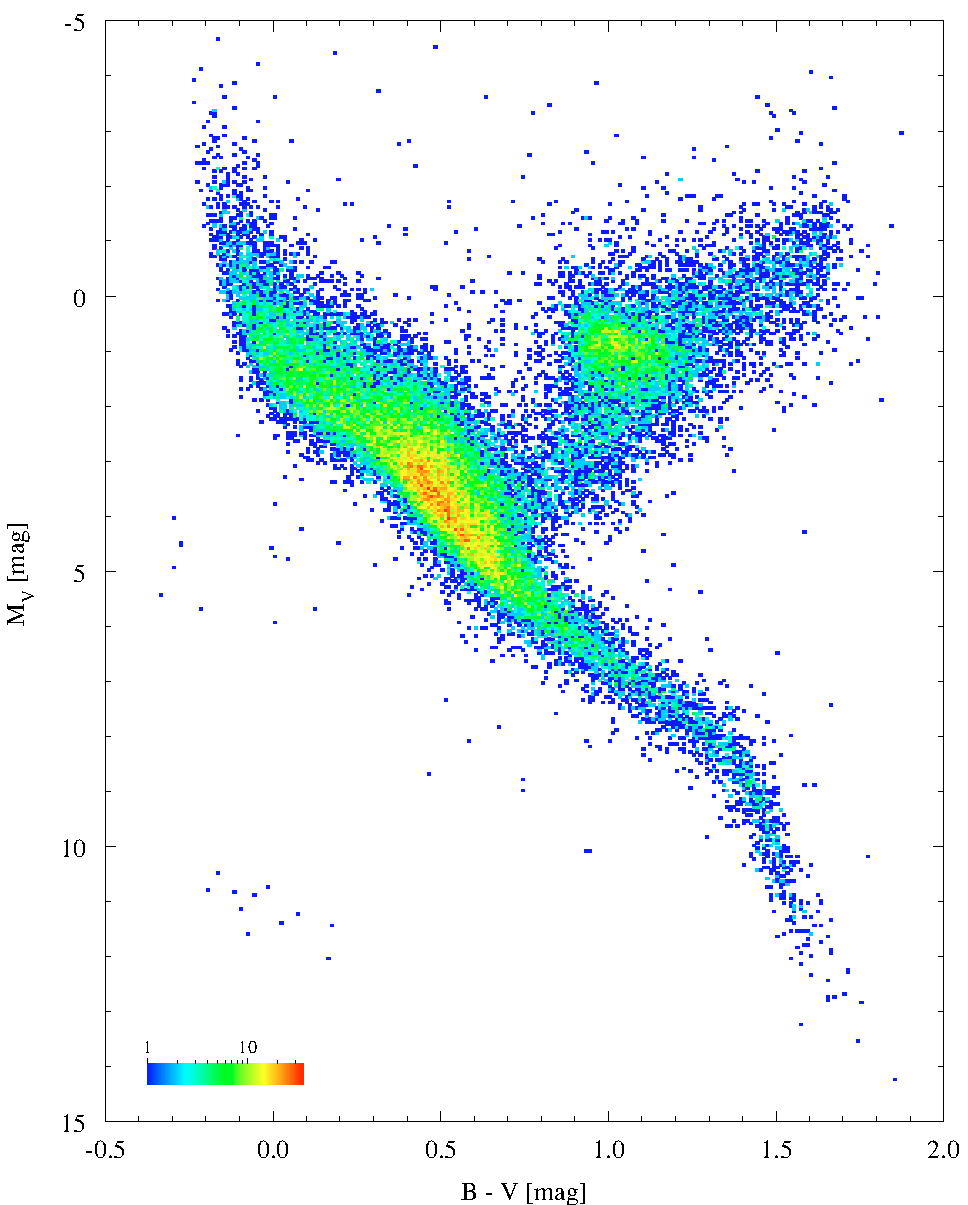
\includegraphics[width=0.75\linewidth]{figures/hr-hip.pdf}
    \caption{Hertzprung-Russel diagram for \(41{,}704\) stars from the Hipparcos Catalogue \citep{Perryman1997}. Colours indicate number of stars in a cell of 0.01 mag in (B-V) and 0.05 mag in V magnitude (\(M_V\)). The main sequence appears as the continuous region extending from the top-left corner of the figure, to the bottom-right corner. The blob above the main sequence, in the top-right region, corresponds to stars in a giant state that have moved out of the main sequence.}
    \label{fig:hr}
\end{figure}

These stars are stable and in a state of \emph{hydrostatic equilibrium}, where gravitational and pressure forces exactly balance each other. The equation of hydrostatic equilibrium is simply the conservation of momentum with zero velocity, \(\fvec{u} = 0\),
\begin{equation}
    \nablavec P = - \rho \nablavec \phi \punct{,}
\end{equation}

which in spherical symmetry can be written as
\begin{equation}
    \frac{\upd P}{\upd r} = - \rho \frac{Gm}{r^2} \punct{,}
\end{equation}

where \(r\) is the distance from the centre of the star and \(m = m(r)\) is the enclosed mass. Together with a description of the composition and nuclear processes taking place in the stellar interior, this gives the complete structure of a star on the main sequence, and is an essential result of the theory of stellar structure.

\subsection{Late stages} \label{sec:star_late}

Every star on the main sequence is supported against gravity by the fusion of hydrogen taking place deep in their core. This process can last from a few million years, to several billion years depending on the mass of the star. The more massive a star is, the faster it will burn its hydrogen. For instance, a star like the Sun is expected to stay on the main sequence for about \(10\) billion years, whereas a star \(50\) times more massive would only last \(\sim3\) million years.

When the core begins to exhaust its available supply of hydrogen, nuclear processes start to slow down. The core thus loses pressure support and contracts under gravity. The star then moves away from the main sequence, and the outcome is once again highly dependent on the total mass of the star.

\subsubsection{Low-mass stars} \label{sec:star_late_lowmass}

Stars of less than about \(8\sunmass\) form a helium core that contracts slowly while the temperature rises in a shell around it. The fusion of hydrogen then moves to this outer shell, leading to an expansion of the star's envelope, but the core stays too cold for helium to burn and continues to collapse on itself. The expansion of the envelope transforms the star into a \emph{red giant}, which can be as large as \(10\text{-}100\sunrad\).

As the core contracts to higher densities, it becomes degenerate, preventing it from collapsing further. This is a consequence of Pauli's exclusion principle, a quantum mechanical effect that forbids fermionic particles, such as electrons, to occupy the same quantum state simultaneously. Because the density has become so high in the core, the electrons are forced to occupy states of higher energy, generating a large pressure. The electron degeneracy pressure can be obtained from the total energy of the free electrons treated as a Fermi gas in the non-relativistic limit (see \citealt{Longair2011} for a complete derivation), and is defined as
\begin{equation}
    P_e = \frac{h^2}{20 m_e} \left( \frac{9}{\pi^2} \rho_e^5 \right)^{1/3} \punct{,}
\end{equation}

where \(h\) is the Planck constant, \(m_e\) the electron mass and \(\rho_e\) the mass density of free electrons in the gas. Electron degeneracy pressure is however independent of the temperature, and stars of \(1\text{-}2\sunmass\) can still reach a temperature high enough for helium burning to take place in the degenerate core with effectively no increase in pressure, while the energy released by the onset of helium fusion further increases the temperature. The consequence is a runaway reaction that fuses most of the helium into carbon over a very short period of time. The large amount of energy released by this reaction can be detected observationally as a \emph{helium flash}.

Stars of higher mass can trigger helium burning before the core reaches degeneracy, therefore producing no helium flash. However, the final outcome stays mostly similar: the contractions of the core will cause the star to \emph{gently} eject its outer layers into a planetary nebula, until only the degenerate core remains. This stellar remnant, known as a \emph{white dwarf}, has a mass of \(0.5\text{-}1.3\sunmass\) and a size comparable to that of the Earth, with a radius of \(\sim6{,}000\units{km}\). It produces no more fusion, and cools down over time.

\subsubsection{Massive stars} \label{sec:star_late_massive}

We henceforth refer to \emph{massive stars} as stars with masses above \(8\text{-}10\sunmass\). These stars burn hydrogen much faster, and the resulting, significantly more massive, helium core collapses much more rapidly than for their lower-mass counterparts. As the pressure and temperature rise quickly, the core reaches helium burning temperatures long before becoming degenerate. This fusion of helium into carbon continues to power the star's core while hydrogen burning moves to a shell around the core that is still hydrogen-rich. Helium depletes much faster than hydrogen, causing the core to collapse once again, until crossing the threshold for carbon and oxygen burning to take place, pushing helium and hydrogen burning further out into the shell. The core undergoes successive phases of fuel exhaustion, during which it further contracts, leading to the burning of heavier and heavier elements while the lighter elements are still burned in a shell structure. This process culminates with the fusion of silicon into iron-group elements, primarily iron and nickel. Since the fusion of these elements is endothermic, the iron produced from the silicon-burning shell does not burn, but rather accretes in an inert core, which quickly becomes degenerate. The final structure of the star is schematised in \Cref{fig:shell_burning}.

Observationally, the star has evolved into either a \emph{red supergiant} or \emph{blue supergiant}. The large amount of energy released by shell burning has caused the outer layers to expand to \(100\text{-}1{,}000\sunrad\), which in turn cools the gas in the envelope. If the star has kept most of its hydrogen envelope, this leads to relatively cold surface temperatures of \(3{,}000\text{-}5{,}000\units{K}\), therefore showing as a red supergiant. However, the envelope becomes more loosely bound to the star, and can easily be ejected by mass-loss processes or gravitational interaction with a binary companion. If the envelope gets ejected, the star evolves into a slightly less large blue supergiant, with surface temperature of \(10{,}000\text{-}50{,}000\units{K}\).

At the final stage of this evolution, the star has completely exhausted its fusion possibilities, and will accumulate iron in its core until it exceeds the Chandrasekhar mass, the limit that can be supported by degenerate electrons. At this point, the iron core typically has a diameter of \(\sim3{,}000\units{km}\) and an average density of \(\sim10^9\units{g/cm^3}\). Nothing can further prevent the core from collapsing, leading to the formation of a neutron star that can either evolve into a black hole if there is enough accretion, in which the entire star eventually falls, or result in a supernova explosion. This is further discussed in \Cref{sec:ccsne}.

\begin{figure}[ht!]
    \centering
    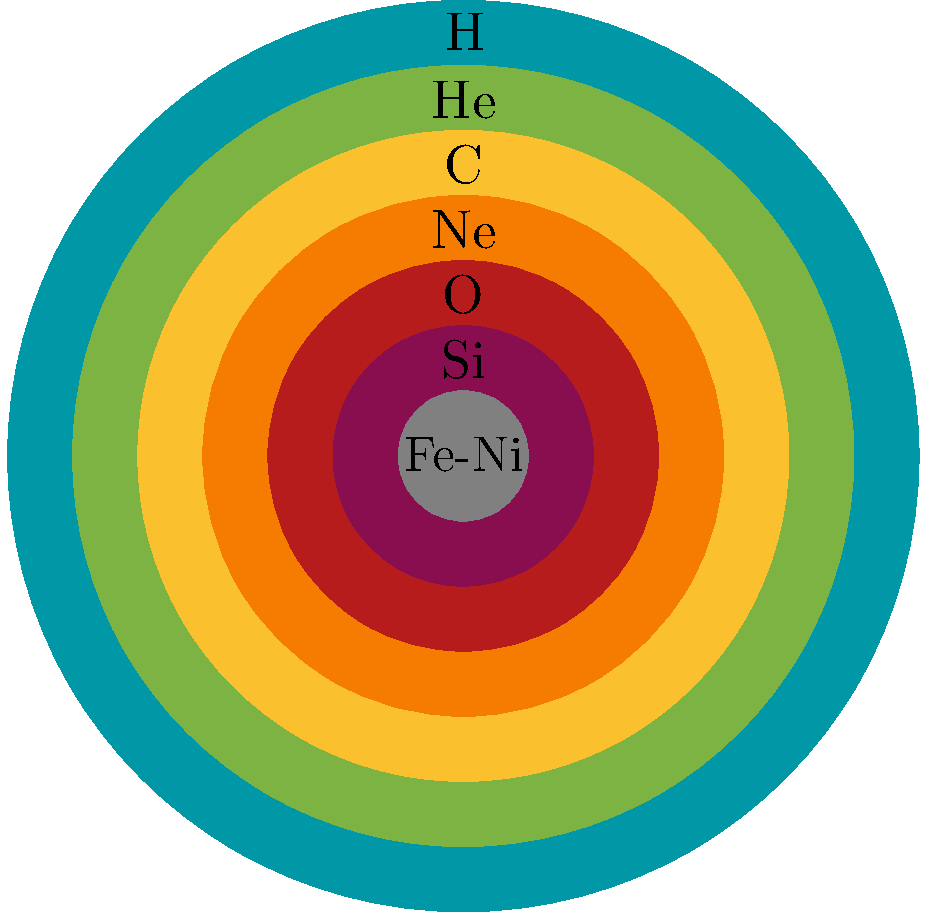
\includegraphics[width=0.5\linewidth]{figures/shell.pdf}
    \caption{Schematic representation of the shell structure of a massive star before the onset of core-collapse. Iron-group elements have accumulated in an inert core at the centre of the star, while lighter elements continue to burn in the outer layers.}
    \label{fig:shell_burning}
\end{figure}

\section{Supernovae} \label{sec:sne}

As we have seen, the late stages of a star's life cycle highly depend on its mass, with the more massive stars exploding as supernovae. We refer to the original object as the \emph{progenitor}. It is the star at the end stage of stellar evolution that leads to the supernova explosion. It can be a single star, or the result of the interaction of multiple stellar bodies. Different progenitors can give rise to very different observable results. In this section, we further define what supernovae are, and discuss both the observational and theoretical properties that characterise them.

\subsection{Observational properties} \label{sec:sne_obs}

Supernovae are transient events, meaning that they can be observed on a human timescale, and can last from a few weeks to several months or even years. They are amongst the most energetic events in the Universe, and can be as bright as an entire galaxy, from millions to billions of times the luminosity of the Sun. Observations of Galactic supernovae, i.e. exploding in our own Milky Way, were already reported by early astronomers of the 11th century and were visible in plain day \citep{Hamacher2014}. This includes, for example, SN 1006 in the Lupus constellation, and SN 1054 whose remnant can still be observed in the Taurus constellation, only \(2\units{kpc}\) away from the Earth, as the well known Crab nebula. The last recorded Galactic supernova was Kepler's supernova in 1604, that exploded about \(6\units{kpc}\) from the Earth, and could be observed with the naked eye. Other unobserved Galactic supernovae were discovered from their remnants, such as Cassiopeia A, estimated to have occurred around 1660-1680 CE \citep{Fesen2006}, \(\sim3.4\units{kpc}\) away from Earth.

It is currently estimated that on average \(\sim1\text{-}3\) supernovae take place per century in a single galaxy \citep{Rozwadowska2021}, therefore the chances of capturing a Galactic supernova are understandably low. Nonetheless, observations of extragalactic events have continuously improved, and automated surveys such as the Zwicky Transient Facility (ZTF) now detect hundreds to thousands of supernovae every year \citep{Fremling2020}.

Supernovae are historically classified according to their observational properties, such as light curves and absorption lines appearing in their spectra. A first classification of supernovae was proposed by \cite{Minkowski1941}, designating supernovae showing hydrogen lines in their spectra as Type II, and those lacking hydrogen lines as Type I. It was then realised that the latter category showed inconsistencies when looking at helium and silicon lines. This category was therefore divided into Type Ia, bearing silicon lines, and Type Ib and Ic, without silicon lines. Type Ib then further shows the presence of helium lines whereas Type Ic does not. \Cref{fig:sn_curves} shows example spectra corresponding to these different classifications. Type II was also further extended into, notably but not exclusively, Type II-P and Type II-L depending on properties of the light curve. After reaching a peak in luminosity, Type II-P supernovae experience a period of nearly constant brightness, a plateau, that can last for about 100 days. On the contrary, Type II-L supernovae show a continuous, almost linear decline of their brightness over time. See \cite{Cappellaro2001} for a more detailed discussion on the supernova classification scheme.

\begin{figure}[ht!]
    \centering
    %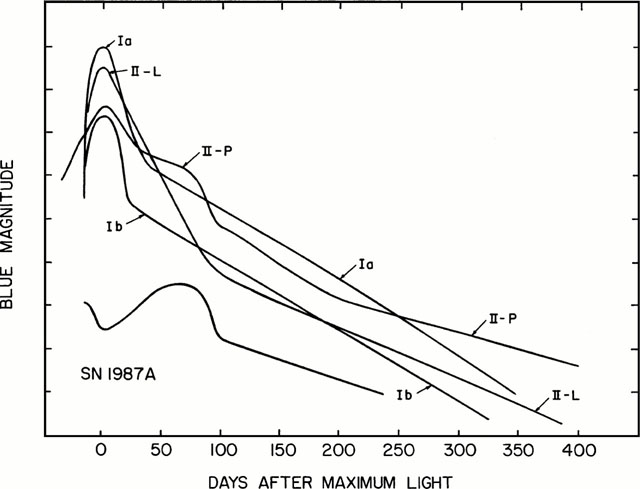
\includegraphics[width=0.75\textwidth]{figures/sn_curves1.jpg}
    %\caption{Typical light curves for different types of supernovae, along with the light curve of SN 1987A. Figure taken from \cite{Filippenko1997}.}
    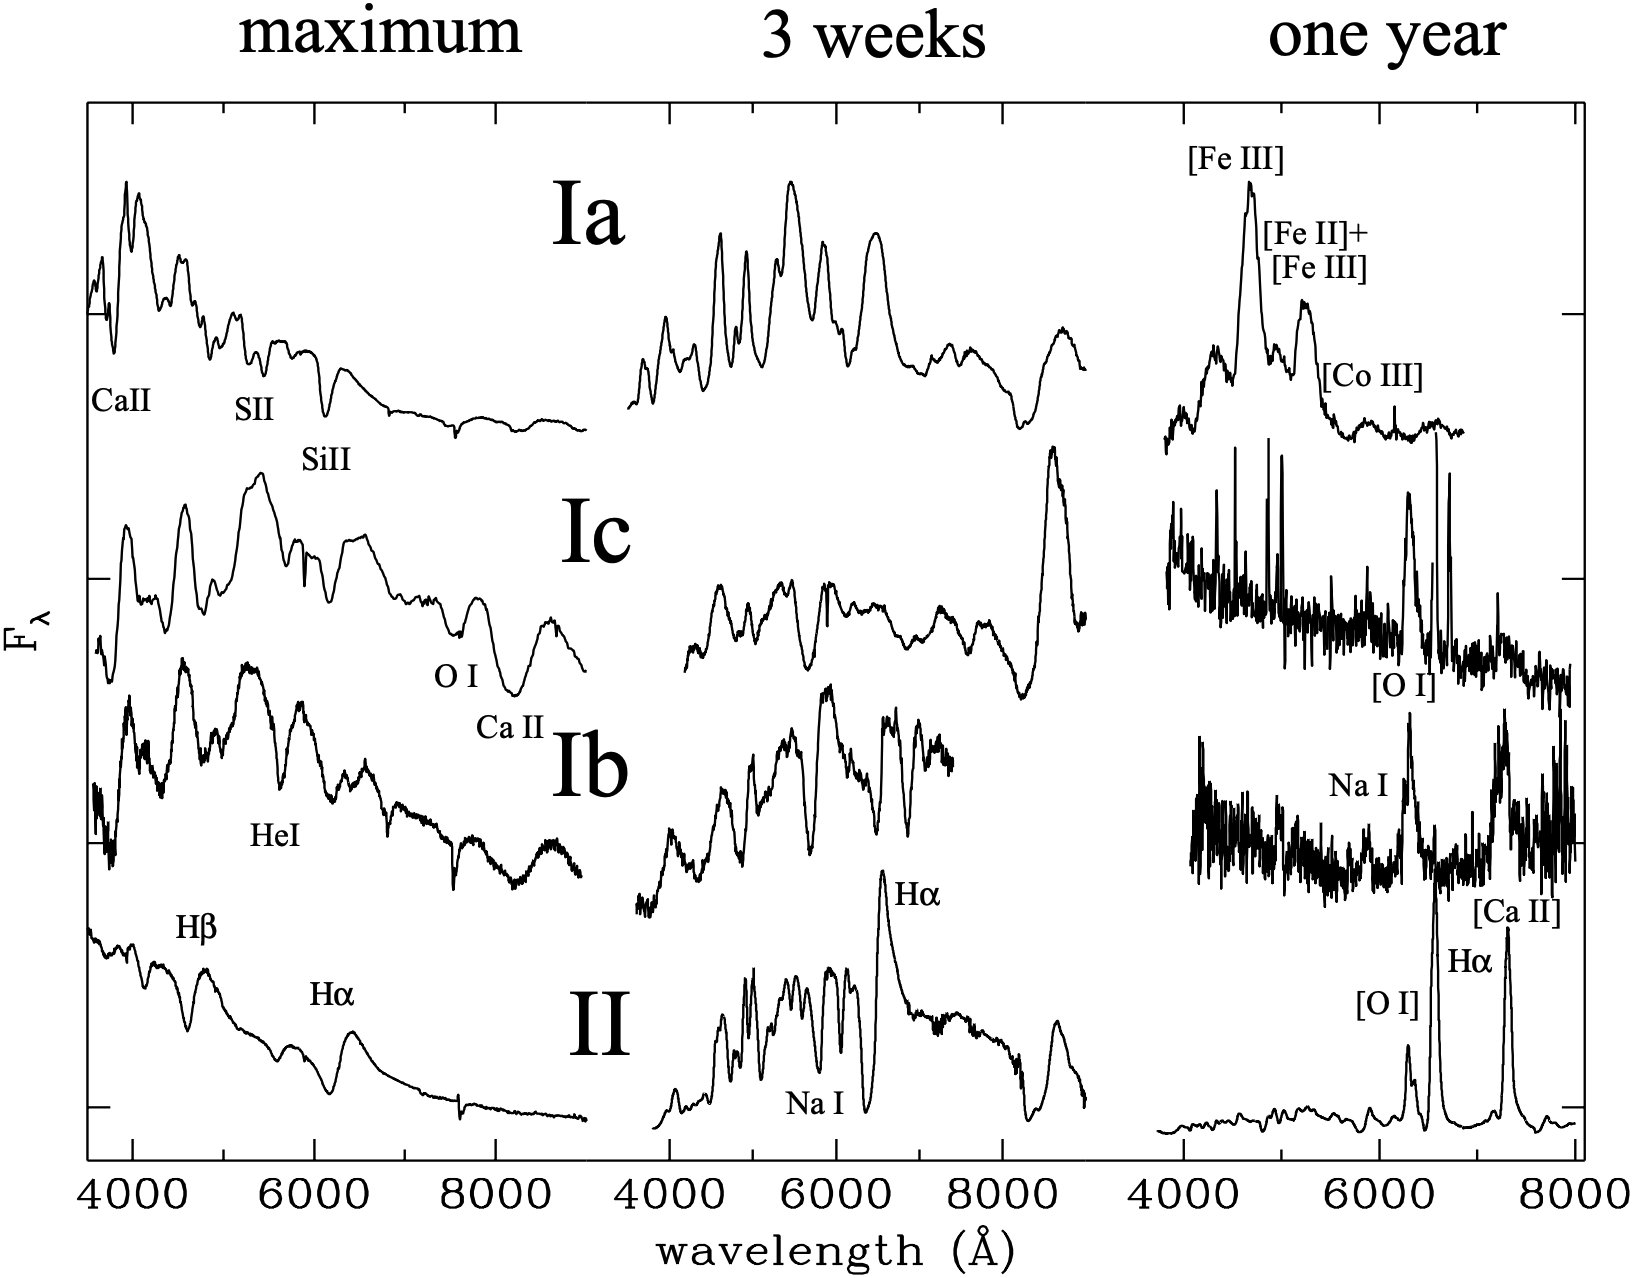
\includegraphics[width=0.75\textwidth]{figures/sn_curves.png}
    \caption{Representative spectra for Type Ia, Ib, Ic and II supernovae, at peak luminosity (left), 3 weeks after (middle) and 10 months after (right). Figure taken from \cite{Turatto2003}.}
    %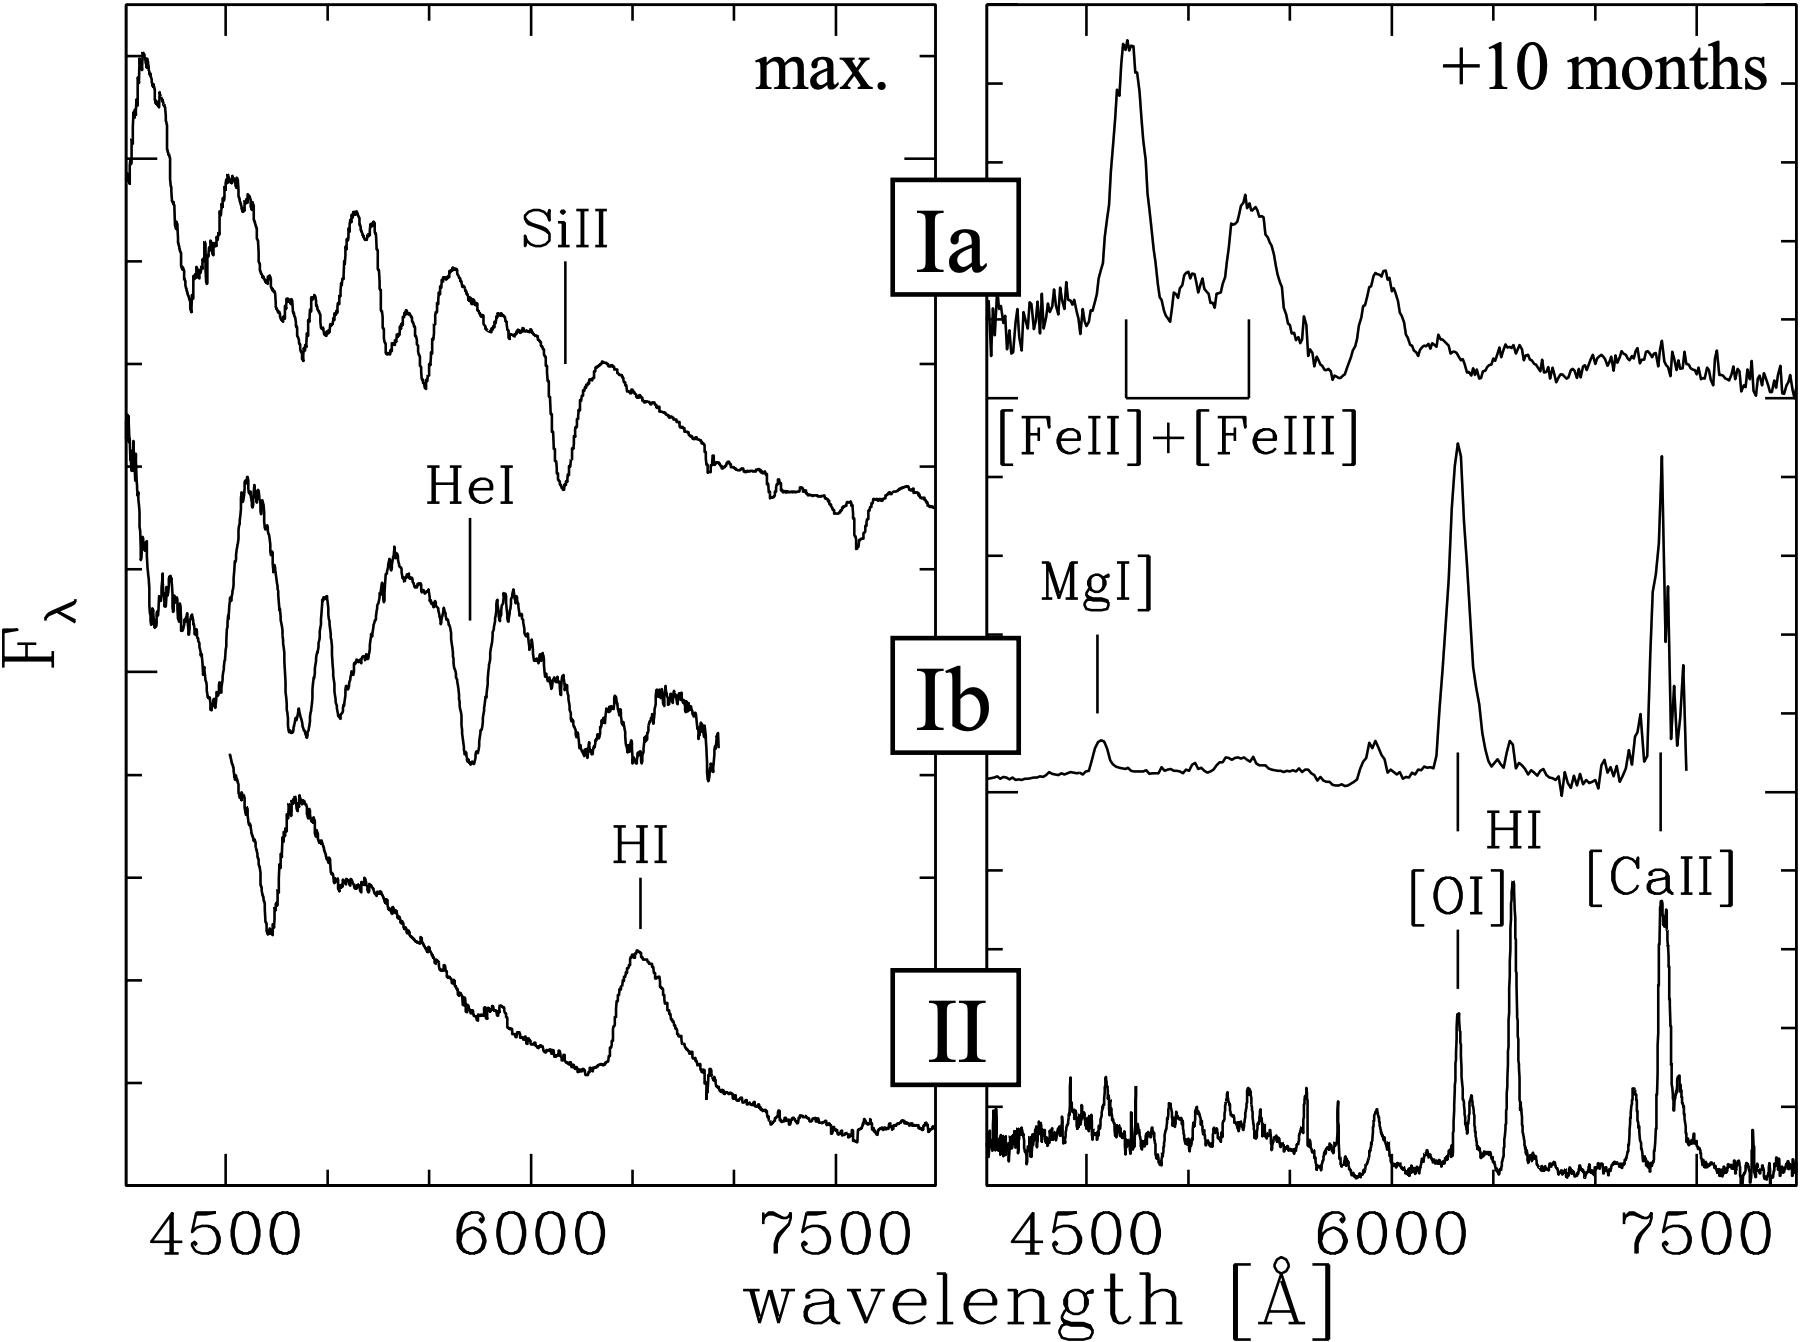
\includegraphics[width=0.75\textwidth]{figures/sn_curves2.png}
    %\caption{Representative spectra for Type Ia, Ib and II supernovae, at peak luminosity (left panel) and at 10 months after (right panel). Figure taken from \cite{Cappellaro2001}.}
    \label{fig:sn_curves}
\end{figure}

\subsection{Explosion mechanism} \label{sec:sne_exp}

From a theoretical point of view, we adopt another approach at classifying supernovae based on the explosion mechanism. The observational classification of supernovae is easily subject to factors such as stellar winds, interactions with the circumstellar medium or evolution in multiple systems, explaining the large amount of subcategories due to altered observable properties. Conversely, a classification based on the explosion mechanism leads to mainly two, well defined, categories: \emph{thermonuclear} and \emph{core-collapse supernovae}. We should note however that the term \emph{core collapse} usually refers more specifically to \emph{iron-core collapse}, and that we focus on this particular type in this thesis. However, a category of \emph{oxygen-core-collapse supernovae}, known as \emph{Electron-Capture Supernovae} (ECSNe), exists and is briefly discussed as well in this section.

\subsubsection{Thermonuclear} \label{sec:sne_exp_ia}

We have discussed electron degeneracy pressure and noted that it is temperature independent. A degenerate star, such as a white dwarf, that were to exceed the Chandrasekhar limit of about \(1.44\sunmass\) would lose pressure support from degenerate electrons and collapse. The collapse would lead to an increase in temperature that would not be balanced by an increase in pressure, thereby reigniting the star. The nuclear reaction rates would then enter a feedback loop and accelerate exponentially, ultimately disrupting the entire star.

White dwarfs composed of carbon and oxygen, the remnants of low-mass stars, are believed to be the progenitors of Type Ia supernovae, and explode due to the ignition of carbon \citep{Mazzali2007}. It is thought however that the star can ignite before the Chandrasekhar limit is attained, and therefore never actually collapses. Type Ia supernovae are the most commonly detected supernovae, partly due to their very high brightness that allows them to be detected from much farther away. Although it is not clear what causes a white dwarf to accumulate excessive mass, and there is no consensus on the matter, it is usually thought to be the result of accretion from a companion star, typically a red giant or supergiant with a loosely bound envelope, or the coalescence of two white dwarfs.
%\haakon{they can just never agree on which one it is}
These progenitors have the particularity of not leaving any remnant, as the entire star is destroyed.

Another type of thermonuclear supernova is the Pair-Instability Supernova (PISN). Very massive stars (\(\gtrsim 140\sunmass\)) have interiors significantly supported against gravity by photon pressure. Due to the very high temperatures, these photons are mostly in the form of gamma rays, which have the property of interacting with each other to form an electron--positron pair. If the temperature and gamma ray density become high enough, the increasing production of electron--positron pairs will cause a loss of support from radiation pressure and render the star unstable to collapse. This further increases the temperature and accelerates the production of gamma rays, until the ignition of oxygen in a runaway process results in the disruption of the entire star in an extremely energetic supernova, leaving no remnant (see section VII in \citealt{Woosley2002} for a detailed description).

The explosion mechanism of PISNe is perhaps the most well understood theoretical model of supernovae. Paradoxically, no PISN has ever been observed despite being predicted to be \(\sim100\) times brighter than Type Ia supernovae. However, theoretical models of nucleosynthetic yields from PISNe have allowed to confirm their existence from the observation of very metal-poor stars in the Milky Way halo, that would have formed from the ejecta of a PISN in the early Universe \citep{Xing2023}. Some PISN candidates have been reported (\citealt{Schulze2024, GalYam2009} for example) but have never been unambiguously classified as such.
%\haakon{I think come candidates exists, but I am not sure. Maybe one of the observers know, could be cool to throw in a reference to a candidate. The PPI supernovae are also interesting for black hole masses.}

\subsubsection{Core collapse} \label{sec:ccsne}

In \Cref{sec:star_late_massive}, we have discussed the mechanisms that lead to the formation of an inert iron core in massive stars. The degenerate core eventually collapses into a neutron star, an extremely compact object of only \(\sim30\units{km}\) in diameter and with a density comparable to several times that of atomic nuclei of about \(10^{14}\units{g/cm^3}\).

The contraction of the iron core results in two important processes, both of which accelerates the collapse. The first is the increasing rate of photodisintegration of iron-group elements. The high temperature breaks the atomic nuclei into free nucleons and alpha particles, which consumes a large amount of thermal energy, therefore decreasing the pressure. The second is a consequence of the rise in density, that accelerates the rate at which free electrons are captured by protons and nuclei, following the reactions
\begin{gather}
    e^{-} + p \rightarrow n + \nu_e \punct{,} \label{eq:nu_e} \\
    e^{-} + (\mathcal{A}, \mathcal{Z}) \rightarrow (\mathcal{A}, \mathcal{Z} - 1) + \nu_e \punct{,} \label{eq:anu_e}
\end{gather}

where \(p\), \(e^{-}\), \((\mathcal{A}, \mathcal{Z})\) and \(\nu_e\) represents a proton, an electron, a nucleus of atomic mass \(\mathcal{A}\) and atomic number \(\mathcal{Z}\), and an electron neutrino, respectively. The pressure support from degenerate electrons is progressively lost as the core becomes more neutron-rich. The neutrinos produced from the above reactions carry energy away and \emph{deleptonise} the core, effectively reducing the Chandrasekhar mass.

% At higher temperature/density, a population of positrons lead to
%   n + e^{+} \rightarrow p + \bar{\nu_e}
% Also pair processes
%   e^{+} + e^{-} \rightarrow \nu_e + \bar{\nu_e}
% and much more (Urca processes when NS cools)

% There's so much to say omg

When the core reaches nuclear densities, due to the repulsive forces between nucleons, the equation of state of matter stiffens, producing a pressure strong enough to abruptly halt the collapse. However, the high inertia of the collapsing core has caused it to contract beyond the equilibrium point and, as a result, the pressure rapidly pushes the core outwards to restore balance with gravity. The inner region of the iron core then collides with the infalling material from the outer shell, resulting in the formation of a shock wave. This moment is referred to as the \emph{core bounce}.

The shock wave propagates outwards through the supersonically infalling shells of material above. The ram pressure on the shock front and the disintegration of the heavy nuclei into free nucleons causes the shock to quickly lose a significant amount of energy. After only \(\sim100\units{ms}\), the shock begins to stall at about \(100\units{km}\) above the proto-neutron star (PNS).

In order for the shock to be revived and the star to explode in a supernova, additional energy must be deposited in the shock front. We remember that the gravitational potential energy can be expressed as
\begin{equation}
    \mathcal{W} \sim \frac{GM^2}{R} \punct{.}
\end{equation}

Calculating this quantity for a PNS (\(M \sim 1.5\sunmass\) and \(R \sim 30\units{km}\)), we see that the collapse of the iron core releases \(\Delta \mathcal{W} \sim 10^{53}\units{erg}\). This energy is initially transformed into thermal energy resulting in the formation of a hot PNS with initial temperature of a few \(10^{11}\units{K}\). Under such conditions of temperature and density, neutrinos dominate the cooling inside the PNS, until most of the binding energy is converted to neutrinos. Neutrinos are weakly interacting particles, and baryonic matter is mostly transparent to them. However, the density in the PNS is high enough to trap the neutrinos, and it takes time, of the order of seconds, for the neutrinos to diffuse out of the PNS. Once the neutrinos escape the neutrinosphere, the high densities at the shock front then allows a portion of the neutrinos to interact, injecting \(\sim1\%\) of the total neutrino energy released, or about \(10^{51}\units{erg}\), directly behind the shock, in a region called the \emph{gain region}. Although only a small amount of neutrinos interact, this is enough to revive the shock, which will continue to propagate through the envelope and explode the star. This mechanism was proposed by \cite{ColgateWhite1966} and later revisited by \cite{Wilson1985}, now known as the \emph{delayed neutrino-driven explosion mechanism} \citep{Bethe1985}. The shock reaches the surface of the star on a timescale of several hours to a few days, and the photons that were trapped behind escape, becoming visible as either a Type Ib/c or Type II supernova.

It is worth noting that, if neutrinos are assumed to be the driving mechanism behind shock revival, this is largely aided by turbulence and instabilities, such as convection, arising in the gain region due to the neutrino heating \citep{Burrows1995}. For this reason, one-dimensional simulations of CCSNe, that fail to account for these multidimensional effects, do not result in successful explosions for most progenitors, except for some of the lowest mass ones \citep{Kitaura2006}. The determination of the exact processes involved and the consequences of these instabilities is still an active area of research.

\subsubsection{Electron capture} \label{sec:ecsne}

In the mass range of \(8\text{-}10\sunmass\) that separates low-mass stars, that turn into white dwarfs, and massive stars, that collapse into neutron stars and black holes, there exist a transitional category of supernovae known as electron-capture supernovae. \cite{Miyaji1980} initially proposed that stars in this mass range could reach temperatures high enough to initiate carbon burning in their core, but not enough to fuse heavier elements, leading to the formation of a degenerate core composed of oxygen, neon and magnesium (ONeMg core). The collapse of the ONeMg core would then be triggered after reaching densities high enough that electron capture processes on neon and magnesium nuclei become significant. In much the same way that was discussed in the previous section on core collapse, electron capture emits neutrinos, deleptonising the core and reducing its effective Chandrasekhar mass, until the collapse of the core into a neutron star becomes inevitable. Observational evidence of ECSNe was found only recently, and it was suggested that the Crab nebula was most likely due to an ECSN \citep{Hiramatsu2021}.

\section{Simulations} \label{sec:sims}

The inherent inability of conventional telescopes to observe the processes taking place deep in the core of dying stars, and the impossibility to reproduce such extreme conditions of density and temperature in laboratories makes the study of supernova explosions a mostly theoretical field.  By developing theoretical and numerical models of supernovae, it becomes possible to guide observations for clues of certain processes, which in turn provides constraints on the otherwise large theoretical parameter space. As an example, we have mentioned the neutrino-driven explosion mechanism for CCSNe proposed by \cite{ColgateWhite1966} that was later supported by the direct detection of neutrinos from the SN 1987A event that occurred in the Large Magellanic Cloud \citep{Hirata1987, Bionta1987, Burrows1987}. In the same way, numerical models of nucleosynthetic yields from PISNe progenitors have been found to match the abundance patterns of very metal-poor stars in the Galactic halo \citep{Xing2023}.

Researchers have been developing numerical models and performing simulations of CCSNe since the late 1960s. The exponential increase in the available computational power has allowed the inclusion of more and more detailed physics over time, starting from simple, one-dimensional, hydrodynamical models powered by pistons, to multidimensional and multiphysics simulations (see \citealt{Janka2012, Mezzacappa2020, Boccioli2024} for detailed reviews and references). However, the complexity of such simulations present a number of challenges and can lead to extreme computational costs, therefore, approximations must be made. For example, a full Boltzmann transport of neutrinos is prohibitively expensive in most situations, and a majority of state-of-the-art simulation codes rather implement approximations based on, for example, moment schemes, leakage or Monte Carlo algorithms (see \citealt{Foucart2023,Mezzacappa2020_Review} for a detailed description of these algorithms). In a similar way, it was shown that a Newtonian approximation of gravity was not acceptable to simulate the central engine of CCSNe \citep{Muller2012,OConnor2018a}, but approximate general relativistic solutions can be used in order to avoid a complete general relativistic treatment. However, the impact of different assumptions and algorithms on the accuracy of the resulting simulations must be carefully tested and analysed, and informed choices on the parameter space to explore must be made.

The description of supernovae involves physics from many different fields, such as magneto-hydrodynamics (MHD), neutrino interactions and nuclear physics, most of which are active areas of research, each carrying a wide range of uncertainties. As a result, self-consistent simulations of CCSNe are hard to achieve, and results from various groups, using different codes, most often do not agree with each other. Furthermore, the computational cost heavily limits the timescales that can be simulated. Most simulations only focus on the first few hundred milliseconds to seconds after core bounce. Long-term simulations, that can evolve from minutes to hours after bounce and reach shock breakout, are very rare, but are nonetheless essential to link simulations to observations. Moreover, such simulations are of particular interest for studying explosive nucleosynthesis and the final composition of the supernova ejecta. This research is crucial to better understand subjects such as galactic chemical evolution and the origin of heavy elements beyond the iron peak, particularly \emph{r}-process elements (see \citealt{Arcones2023} for a review). 
In this work, we have explored the achievability of long-term simulations of CCSNe at a reasonable computational cost based on the formation of a neutrino-driven wind around the PNS in the first seconds after bounce. We do so by excising the central region of the star, where the PNS is located, and replacing it with an inner boundary condition that mimics this neutrino wind. This method is presented in \Cref{chap:methods}.

\section{Neutrino-driven winds} \label{sec:ndw}

At the moment of collapse, the gravitational binding energy released by the formation of the PNS is transformed into thermal energy. The high temperatures inside the PNS trigger nuclear processes that convert most of this energy into neutrinos. However, these neutrinos are originally trapped inside the PNS due to the high densities, and slowly diffuse through the inner core before escaping the neutrinosphere, carrying away energy and cooling the neutron star. The neutrinosphere is the region outside the PNS that presents steep gradients in density and temperature, and where the mean free path of the neutrinos become comparable to the size of the PNS. A fraction of the escaping neutrinos interact with matter in this region, following the inverse reactions of \Cref{eq:nu_e,eq:anu_e}, depositing energy that blows off matter from the surface of the neutron star. If no matter is being accreted on the PNS, this outflow can become supersonic and form a \emph{neutrino-driven wind}. This neutrino-driven wind is usually characterised by a relatively smooth, quasi-spherically symmetric profile, forming \(\sim1\units{s}\) after bounce. At this point, the shock has been successfully launched and has propagated to sufficiently large radii (\(\sim10{,}000\units{km}\)) that it has little to no effects on the conditions in the region of interest. The PNS, however, continues to cool on the Kelvin-Helmholtz timescale for a few tens of seconds after the explosion. During this period, the neutrino luminosities and the properties of the neutron star (mass, radius and temperature) change very slowly. This description was supported by simulations by \cite{Janka1995}, and allows us to express the hydrodynamics of the outflow using a quasi-steady state approximation, so that mass, momentum and energy conservation can be written in spherical symmetry as
\begin{gather}
    \dot{M} = 4 \pi r^2 \rho u \punct{,} \\
    u \frac{\upd u}{\upd r} = - \frac{1}{\rho} \frac{\upd P}{\upd r} - \frac{GM}{r^2} \punct{,} \\
    \dot{q} = u \left( \frac{\upd \mathcal{E}}{\upd r} - \frac{P}{\rho^2} \frac{\upd \rho}{\upd r} \right) \punct{,}
\end{gather}

where \(\rho\), \(P\), \(u\) and \(\mathcal{E}\) denote the density, pressure, flow velocity and specific internal energy, respectively, and \(M\) is the mass of the neutron star, \(\dot{M}\) is a constant mass outflow rate, and \(\dot{q}\) is the specific heating rate due to neutrino interactions. Note however that the pressure and specific internal energy accounts for non-relativistic nucleons as well as relativistic particles (electrons and positrons) and photon radiation. This description of the neutrino-driven outflow from the hot neutron star was first brought forth by \cite{Duncan1986}.

In reality, the conditions in the wind may be more complex, and influenced by late accretion on the PNS, rotation, or continued convection in the gain region. It is however a convenient approximation to explore the impact of the neutrino wind on the nucleosynthesis and dynamics of the inner-most ejecta of the supernova, near the PNS. In particular, the implications of the neutrino-driven wind as a potential site of production of heavy elements by rapid neutron capture, known as \emph{r}-process, have been under investigation since the early 1990s. Under the steady state assumption, \cite{Qian1996} identified the key parameters characterising the neutrino wind that describe the nucleosynthesis in the ejecta: the mass loss rate, the entropy per baryon, the expansion timescale and the electron fraction. The latter parameter, the electron fraction, is defined as
\begin{equation}
    Y_e = \sum_i \left( \frac{Z_i}{A_i} \right) X_i \punct{,}
\end{equation}

where \(Z_i\), \(A_i\) and \(X_i\) are the atomic charge, mass number and mass fraction of species \(i\), respectively. It is used to define whether the ejecta is neutron-rich (\(Y_e < 0.5\)) or proton-rich (\(Y_e > 0.5\)), and is importantly influenced by neutrinos, where the competing interactions of electron neutrino and antineutrino capture usually renders the wind more proton-rich in the context of neutrino-driven supernovae. As a consequence, a strong \emph{r}-process in the neutrino wind does not seem possible in neutrino-driven supernovae. However, a weak \emph{r}-process is possible and can contribute to the formation of the lighter heavy elements, from strontium to silver \citep{Arcones2014}. In the case of more proton-rich conditions, another process known as the \(\nu p\)-process can take place \citep{Frohlich2006,Nevins2024}. Furthermore, exotic supernovae such as magneto-rotational supernovae and collapsars, are thought to be potential sites of strong \emph{r}-process. Although the subjects of nucleosynthesis and explosive burning in CCSNe are not further developed for the purpose of this thesis, they are nonetheless essential aspects of this field, and we refer the interested reader to \cite{Arcones2013, Boccioli2024} for reviews.
